\clearpage

\section{Methodology}

\noindent
\begin{enumerate}
    \item Dataset: 
    Common data sets cannot be trained to recognize the objects on the water's surface.  We have used the Flow Dataset for floating waste objects, this dataset contains 2000 images with 5271 floating wastes like plastic bottles and drinking cans. We have done a balanced Train-Validate-Test Split. Along with images dataset also contains 200 sequence videos for training. The interval of the video varies from several seconds to a minute. Each video contains almost 1-8 floating waste instances. 	We have converted this raw video into images by extracting the frames. Our dataset contains more small objects, which makes it challenging for detection.

\item Base Model Architecture Selection:
In this project, as we are using the concept of distillation, we require two models the first one is the base model, and the other one is the target model. As annotating data is very time and money-consuming, We are using GroundedSAM as a base model, automatically annotating the images we have taken from the FloW dataset. GorundedSAM uses grounding DINO to detect and label the images and uses the Segment Anything Model to generate the masks of images. So by combining the power of DINO, GLIP, and SAM, we can automatically annotate our data.


\item Dataset preparation:
The base model GroundedSAM will take raw images and videos as input along with the proper ontology to annotate the data to produce the auto-label dataset automatically. This dataset can be used to train the target YOLOv8 model.
As we need to compare the results of distillation from GroundedSAM to YOLOv8 and the performance of training YOLOv8 without distillation, We preprocessed the dataset by resizing images to a consistent resolution, normalizing pixel values, and converting annotations into the YOLOv8-compatible format using Roboflow tool. \textbf{make each of these bullets as just paragraphs with headlines in bold and add citations and references wherever required}


\item Target Model Architecture Selection:
For the target model, We have chosen the YOLOv8 for developing the floating object detection model. YOLOv8 (You Only Look Once v8) is a state-of-the-art object detection model developed by Ultralytics. It is a real-time object detection model that can achieve high accuracy and speed. It is an advanced variant in the YOLO family. YOLOv8 is also a good choice for floating object detection because it is specifically designed to detect objects at different scales. This is important for floating object detection, as floating objects can vary significantly in size. YOLOv8's ability to detect objects at different scales makes it more likely to accurately detect floating objects in images and videos.


\item Distillation:
Although effective, foundation models like GroundedSAM include limitations such as high GPU computation requirements, slow real-time performance, and restricted accessibility. These restrictions prevent its application in low-compute environments, such as edge devices, inhibit the development of original intellectual property, and prevent cost-effective use. Although foundation models have a wealth of information across many fields, many real-world applications of AI demand an in-depth understanding of specific fields. Distillation offers a way to utilize the power of expansive models without direct deployment. It transfers the knowledge of the expensive vase model to the target model without affecting efficiency and accuracy to get a fast and deployment-ready model\cite{Distill}. In this project, we are transferring the knowledge of object detection from GroundedSAM to the YOLOv8 model with the help of the AutoDistill library.


\item Model Training:

The target model YOLOv8 takes the auto-labeled data produced by the GroundedSAM and gives the deployment-ready model for floating waste detection. We have trained the YOLOv8 on both datasets, the one automatically labeled by the groundedSAM and the one labeled manually using the labeling tool.
The cosine Annealing method is used in the training phase of YOLOv8.
Cosine annealing is a learning rate decay strategy that uses a cosine function to decrease the learning rate gradually over time. The learning rate is initialized at a high value and then drops to a lower value throughout training. It helps to produce good results. The deep learning framework is TensorFlow, GPU is Tesla 4, during training, the batch size is set to 16, the training epoch is set to 100, and the learning rate is 0.001. 

\item  
Model Testing: 
The output of the trained model gives us the distilled model, which successfully recognizes floating waste objects in various images. These results show that distillation from GroundedSAM to YOLOv8 is a powerful floating object detection tool model that is accurate, fast, and can detect a wide variety of objects.
\\

\end{enumerate}

\section{Task Completed}
\begin{enumerate}
    \item Image Dataset Preparation: 
    Downloaded the raw images and videos of floating waste objects from the FloW dataset, ensuring that most objects are small. We have split the videos into images by saving the 15th frame from each video. We have also kept videos for evaluating the model.

\item Select the model for floating waste detection:
We have selected the GroundedSAM as a base model and YOLOv8 as a target model.


\item Setup Python environment and Install dependencies: We have set up the GPU environment and installed the required dependencies. As we are using the concept of distillation, we have installed the Autodistill library. And for the base and target models, we have installed Autodistill packages that are required for our chosen models.


\item Define Ontology: 
We have used CaptionOntology. It prompts a Base Model with text captions and maps them to class names. We have defined the Ontology to detect the waste floating on the water's surface, basically plastic bottles and drink cans.


\item Autolabel the images:
We have initialized the base model GroundedSAM with unlabeled input data and ontology to convert into the annotated dataset. As base models are very slow but efficient, take took 2 hours of time time to annotate the data.


\item Display sample of dataset:
The dataset is the result of the GroudedSAM model. This dataset will be used to train YOLOv8. The dataset contains automatically labeled images. We are displaying a sample of data to look at the model's performance.

\item Distillation from base to target model:
We have distilled the knowledge from the base model groundedeSAM to YOLOv8. Now YOLOv8 will consume the auto-labeled data and give a fast and real-time distilled model for deployment.

\item Training of model: 
We have trained the YOLOv8 on auto-labeled and manually annotated data. So that we can compare the results of the training with or without knowledge distillation.

\item Evaluating and Testing the Model:
We have evaluated and tested the model on the FloW dataset.

\end{enumerate}

\section{Experiment and Result Analysis}
This section discusses the results of the project.
% \noindent\\
    % \centering
\begin{enumerate}
\item Sample of data:
\ref{fig:Data} shows the sample from the dataset used as input for the groundedSAM model.

\item Data sample generated by GroundedSAM:
The following \ref{fig:Dataset} shows the outstanding result of GroundedSAM for automatically Annotating the data. It outputs the masks of waste objects from the images.

\begin{figure}[H]
\centering
	\includegraphics*[height=10cm, width = 10cm]{images/Data-Sample.png}
	 \caption{Data Sample}
	\label{fig:Data}
\end{figure}

 \item Training Result:
\ref{fig:t-auto} shows the result of the training YOLOv8 on the auto-labeled dataset generated by the GroundedSAM. This is the result when we just give images and text prompts to the GroundedSAM model and then distill the knowledge from the base model to the target model. It gives 0.741 mAP50. 
\ref{fig:t} shows the result of the training YOLOv8 on the annotated FloW dataset. This is the result when we are giving annotated FloW dataset to YOLOv8. We have trained the YOLOv8 model for 100 epochs from scratch for this custom dataset for a batch size of 16. It gives 0.925 mAP50.
The training results are summarized in the \ref{table:training-1}
\newline

\item Evaluation Result: We have evaluated the distilled model on the 400 validating images. \ref{fig:eval} shows the result of one batch with size 16.\newline 
\begin{figure}[H]
\centering
	\includegraphics*[height=10cm, width = 10cm]{images/Data-Sample-generated-GroundedSAM.png}
	 \caption{Data Sample generated by GroundedSAM}
	\label{fig:Dataset}
\end{figure}


\item Test Results:
While testing, the model clearly shows that it can detect floating waste objects in complex environment situations \ref{fig:test} like reflections and excessive light. The distilled model has given state-of-the-art performance for detecting floating waste objects by taking prompts and images as input. The results are also compared with other models in table \ref{table:training-1} and table \ref{table:training-3}. We have also compared the Speed per image and FPS for YOLOv8 and DistilledFloatNet in table \ref{table:training-2}
% 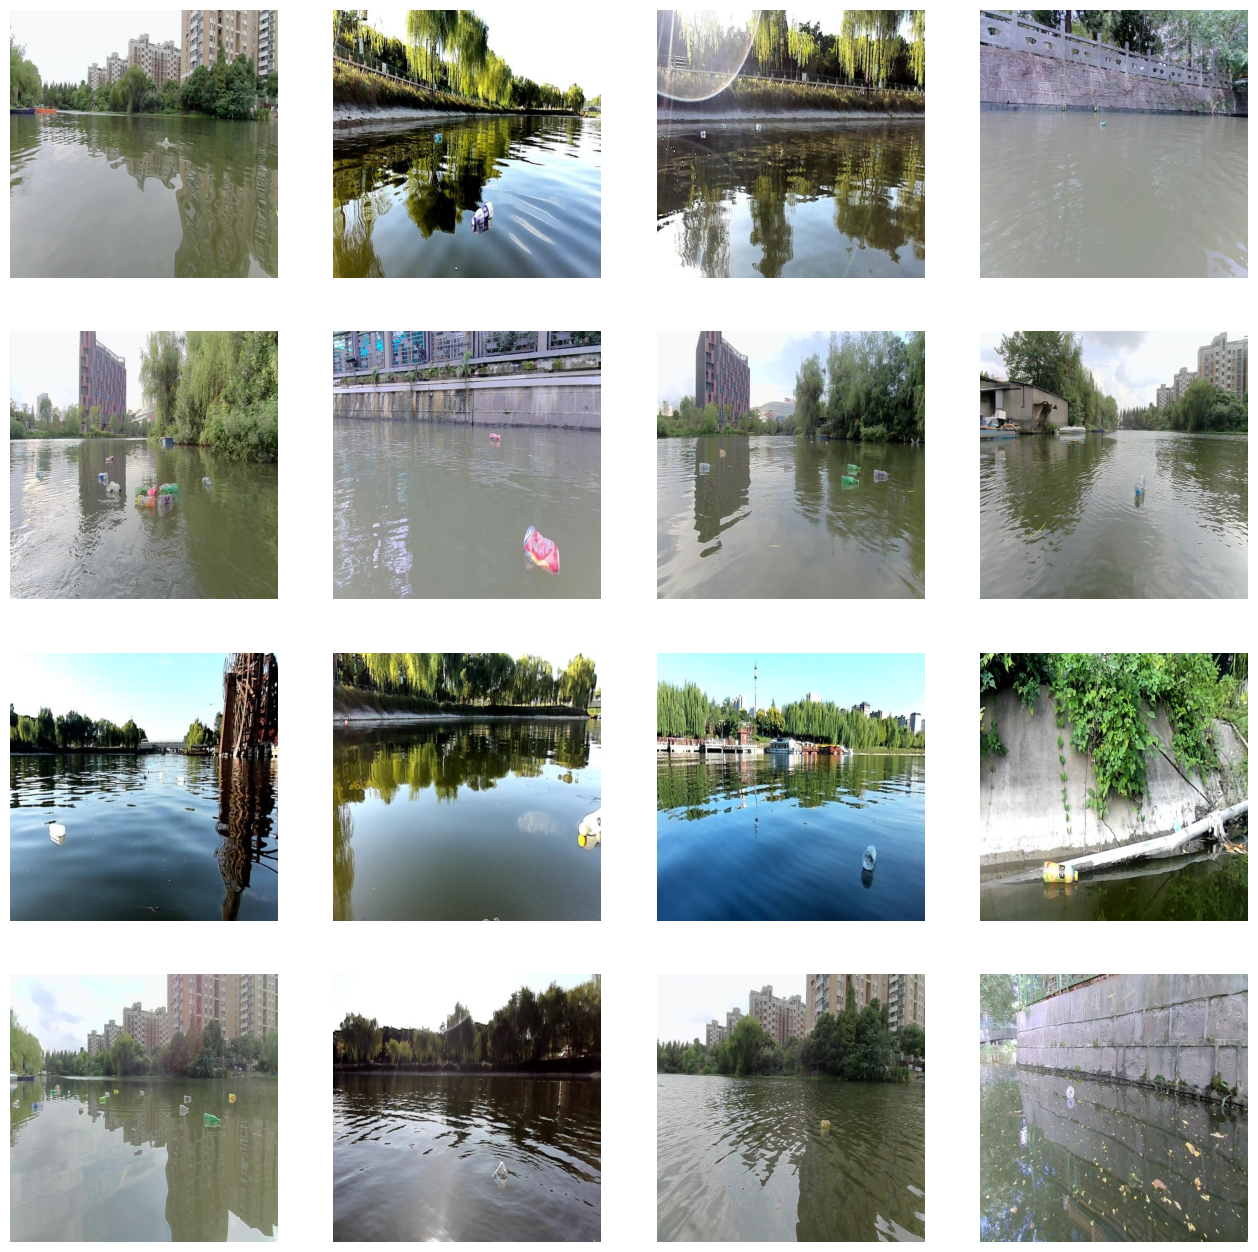
\includegraphics[width=14cm]{images/Data-Sample.png}
% \begin{center}
%     Fig(7) Data Sample
% \end{center}
%  \begin{table}
%     \centering
   
%    \begin{tabular}{ | m{8em}| m{6em} | m{5em} | m{6em} | m{7em}|} 
%         \hline
%         \textbf{Model} & \textbf{Precision\%} & \textbf{Recall\%} & \textbf{mAP50\%} & \textbf{mAP50-95\%} \\
%         \hline
%         GroundedSAM \newline and YOLOv8 \newline using Distillation & 69.9 & 69.5 & 74.1 & 55.4 \\
%         \hline
%         YOLOv8 \newline without\newline using Distillation & 90.9 & 88.5 & 92.5 & 52.2 \\
%         \hline
%     \end{tabular}
%     \centering
%      \caption{Training Results}
%      \label{table:1}
% \end{table}   

\begin{table}
    \centering
    \label{tab:my_label}
\begin{tabular}{lccccr}
\hline \multicolumn{1}{c}{\textbf{Model}} & \textbf{Precision\%} & \textbf{Recall\%} & \textbf{mAP50\%} & \textbf{mAP50-95\%}\\
\hline 
DistilledFloatNet & 69.9 & 69.5 & 74.1 & 55.4\\
YOLOv8 & 90.9  & 88.5 & 92.5 & 52.2 \\
\hline
\end{tabular}
\caption{Training Results}
\label{table:training-1}
\end{table}

% 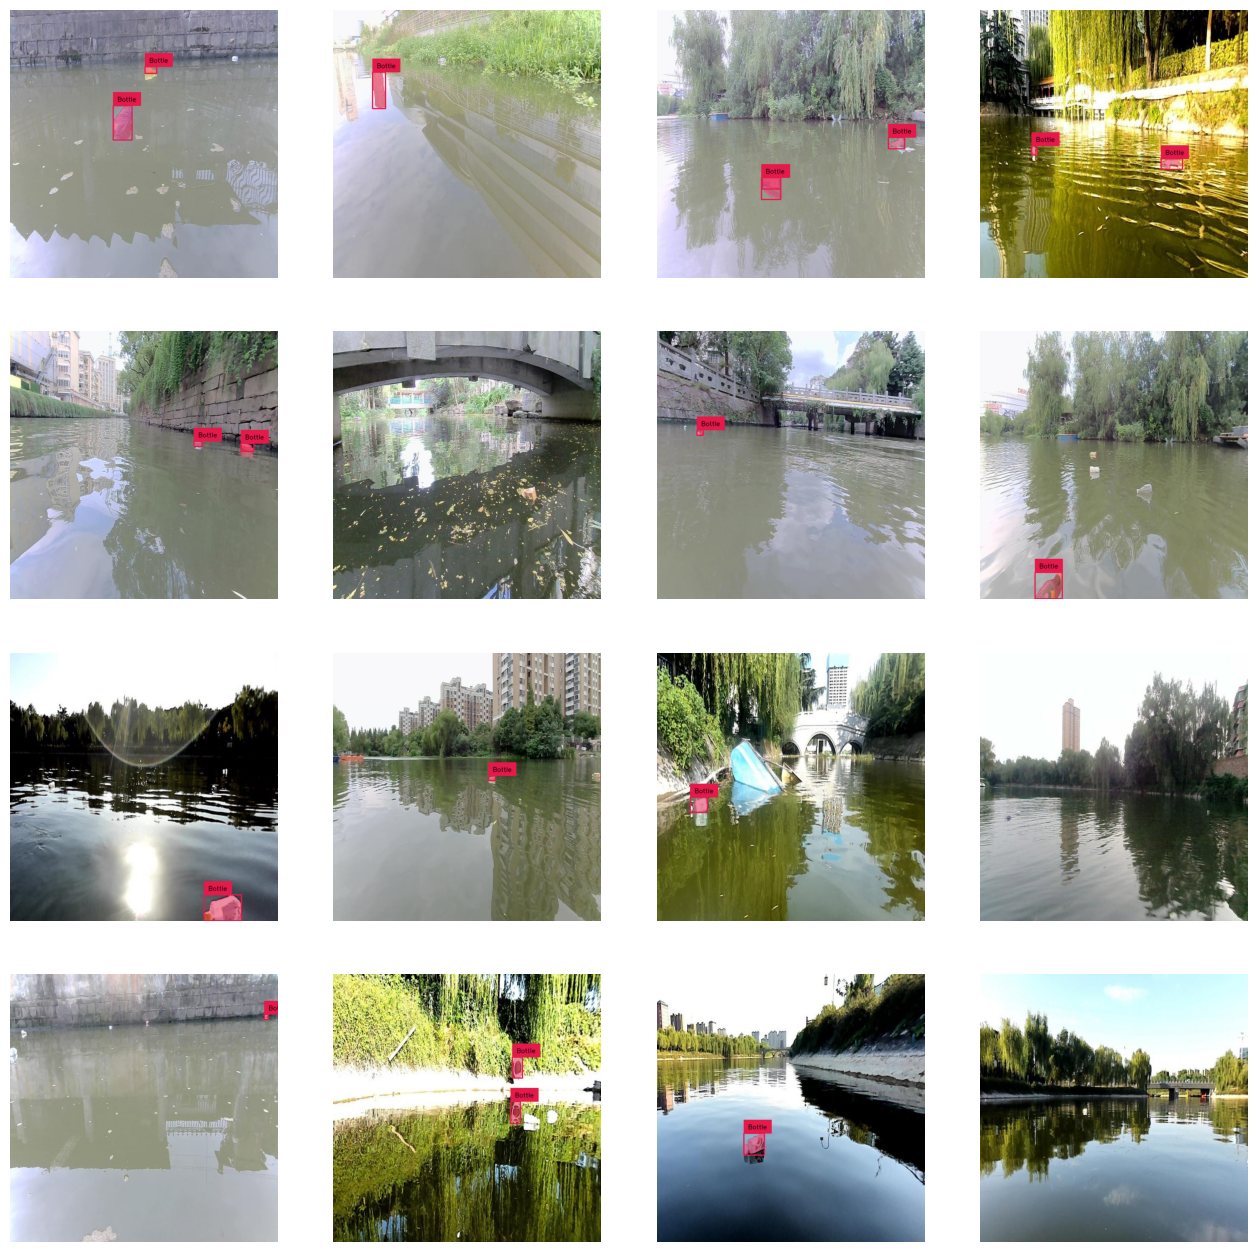
\includegraphics[width=14cm]{images/Data-Sample-generated-GroundedSAM.png}
% \begin{center}
%     Fig(8) Data Sample generated by GroundedSAM
% \end{center}
\vspace{\baselineskip}
\vspace{\baselineskip}

\begin{figure}[H]
\centering
	\includegraphics*[width = 14cm]{images/training-result-with-distillation.png}
	 \caption{Training result with distillation}
	\label{fig:t-auto}
\end{figure}

% 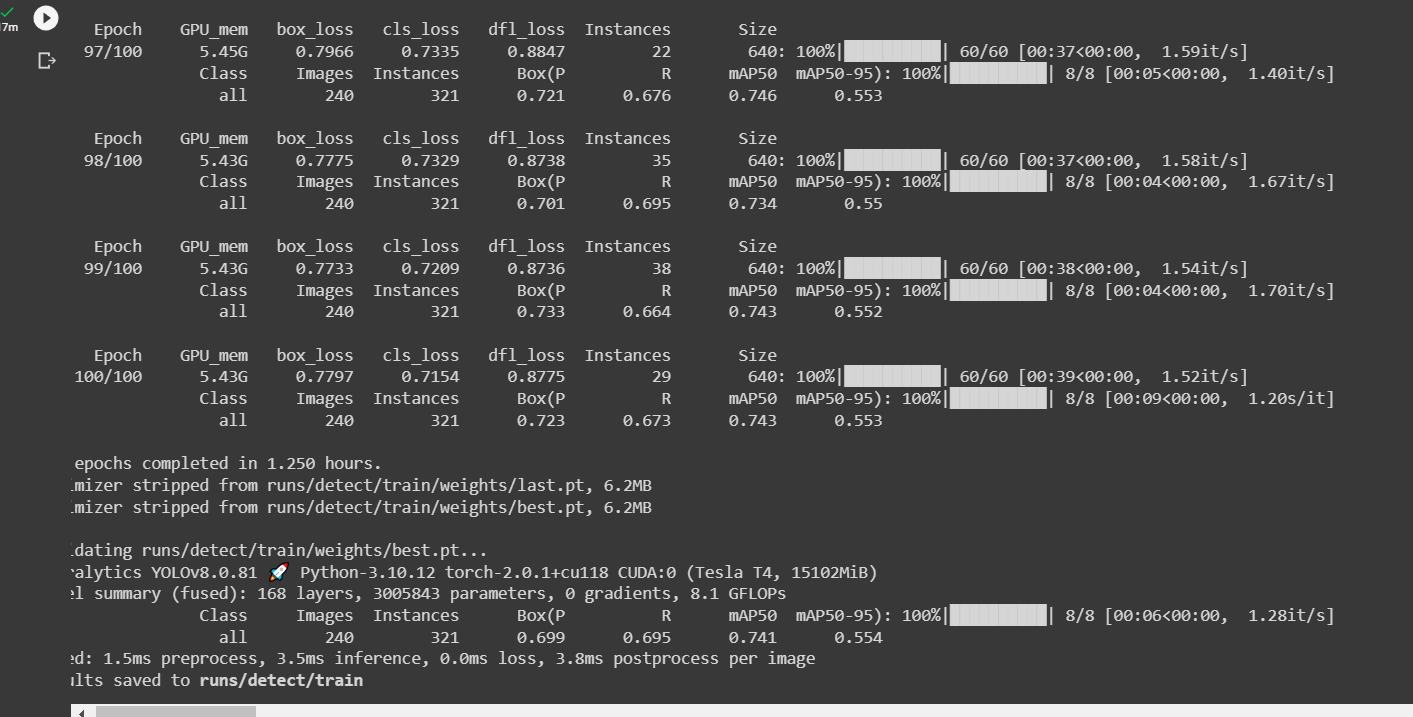
\includegraphics[width=14cm]{images/training-result-with-distillation.png}
% \begin{center}
%     Fig(9) Training result with distillation
% \end{center}
\vspace{\baselineskip}
\vspace{\baselineskip}


\begin{figure}[H]
\centering
	\includegraphics*[width = 14cm]{images/training-result-without-distillation.png}
	 \caption{Training result without distillation}
	\label{fig:t}
\end{figure}

% 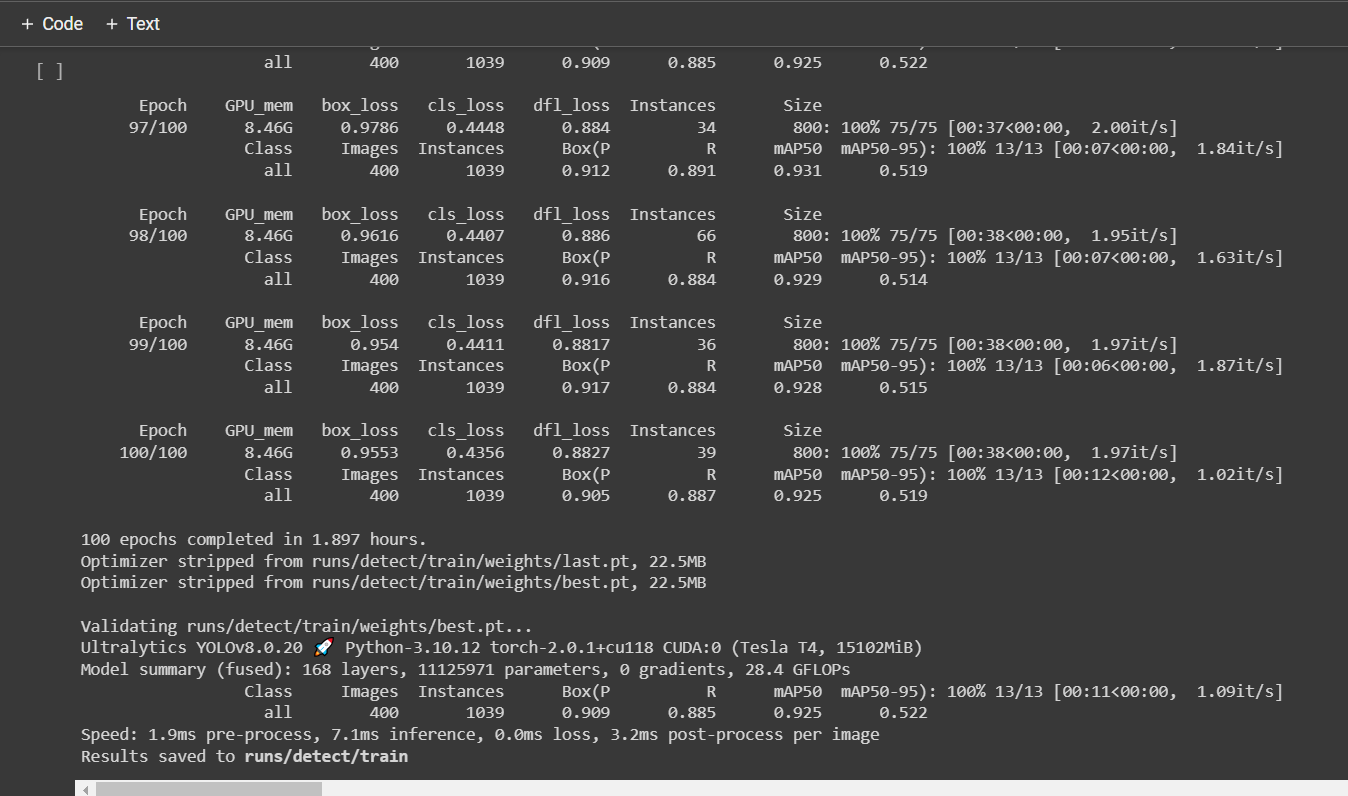
\includegraphics[width=14cm]{images/training-result-without-distillation.png}
% \begin{center}
%     Fig(10) Training result without distillation
% \end{center}
\begin{table}[H]
    \centering
    \label{table:training-2}
\begin{tabular}{lcr}
\hline \multicolumn{1}{c}{Model} & Dataset & mAP50-95\\
\hline 
DSSD & $FloW$ & 27.5 \%\\
RetinaNet & $FloW$  & 24.9 \% \\
YOLO-v3 & $FloW $ & 12.8 \% \\
Faster R-CNN & $FloW $ & 18.4 \% \\
FPN & $FloW $ & 33.4 \% \\
Cascade R-CNN & $FloW $ & 43.4 \% \\
\textbf{YOLOv8} & $\textbf{FloW} $ & \textbf{55.2\%}\\
\textbf{DistilledFloatNet} & $\textbf{FloW}$ & \textbf{55.4 \% }\\
\hline
\end{tabular}
\caption{Comparison with other Models}
\end{table}

\begin{table}[H]
    \centering
   
\begin{tabular}{lccccr}
\hline \multicolumn{1}{c}{Model} & Pre-process & Inference & Post-process & FPS\\
\hline 
YOLOv8 & 0.4ms & 11.9ms & 5.2ms & 57.14\\
DistilledFloatNet & 0.7ms  & 10.0ms & 2.0ms & 78.74 \\
\hline
\end{tabular}
\caption{Speed per image and FPS}
 \label{table:training-2}
\end{table}

\begin{figure}[H]
\centering
	\includegraphics*[height=10cm,width = 10cm]{images/Evaluation_image.png}
	 \caption{Data Evaluation Result}
	\label{fig:eval}
\end{figure}



% \begin{figure}[H]
% \centering
% 	\includegraphics*[height = 9cm, width = 10cm]{images/test-img-1.png}
% 	 \caption{Test Image 1}
% 	\label{fig:test1}
% \end{figure}

% \begin{figure}[H]
% \centering
% 	\includegraphics*[height = 9cm, width = 10cm]{images/test-image-2.png}
% 	 \caption{Test Image 2}
% 	\label{fig:test2}
% \end{figure}

% \begin{center}
% 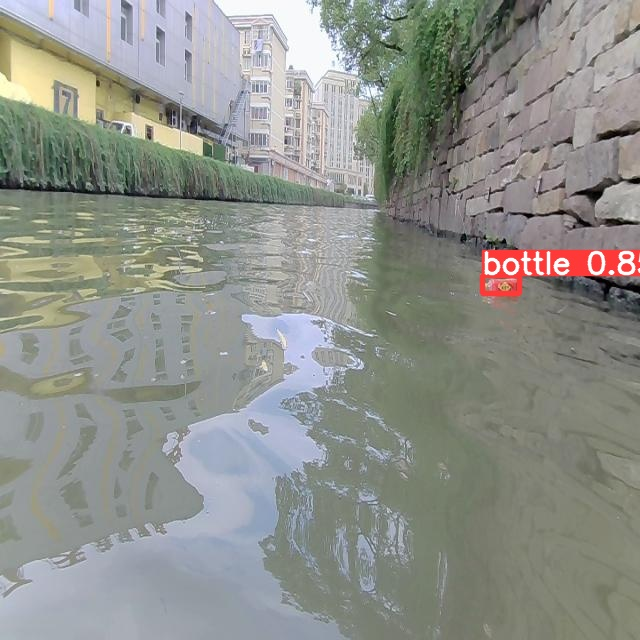
\includegraphics[width=10cm]{images/test-img-1.png}
% \begin{center}
%     Fig(12) Test Image 1
% \end{center}
% \end{center}

% \begin{center}
% 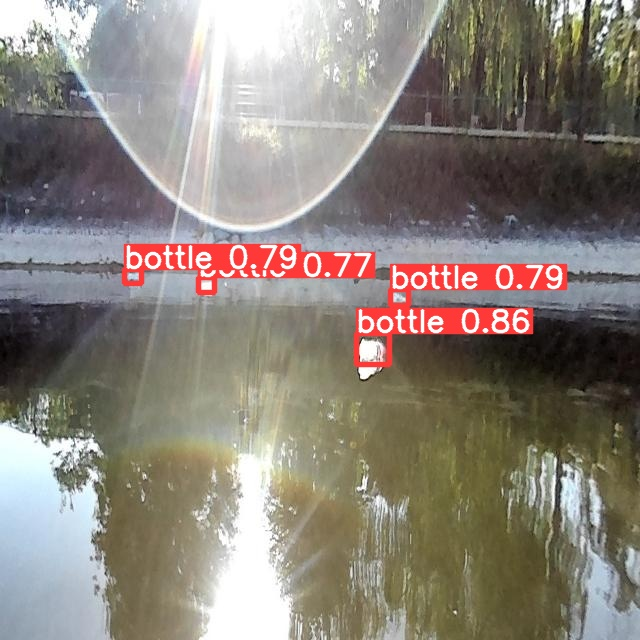
\includegraphics[width=10cm]{images/test-image-2.png}
% \begin{center}
%     Fig(12) Test Image 2
% \end{center}
% \end{center}

\item Loss Functions:
The loss functions are used to train the YOLOv8 model. For Bounding-Box loss, YOLOv8 uses the CIoU and DFL loss functions and BCE for class loss. These losses have increased object identification performance, especially with small objects. The model is trained to minimize the loss function. The loss functions can be used to analyze the performance of the YOLOv8 model. The lower the loss function, the better the model is performing. The loss functions can also identify areas where the model performs poorly. We have Monitored the loss functions during training in \ref{fig:r1} and \ref{fig:r2}: 
\begin{enumerate}
    \item The train/box-loss curve is a decreasing curve. This means that the box loss decreases as the model trains. A decreasing box loss indicates that the model is learning to predict the bounding boxes more accurately.
    \item The train/cls-loss curve is decreasing curve. This means that the cls-loss falls as the model trains. A decreasing cls-loss indicates that the model is learning to predict the classes more accurately.
    \item The dfl-loss curve is a decreasing curve. This means that the dfl-loss decreases as the model trains. A decreasing dfl-loss indicates that the model is learning to handle class imbalance better.
    \item The val/box-loss curve is a decreasing curve. This means that the val-box-loss decreases as the model validates. A decreasing val-box-loss indicates that the model is learning to predict the bounding boxes more accurately.
    \item The recall curve is an increasing curve. This means that the recall increases as the model trains. An increasing recall indicates that the model is becoming more confident in its predictions. This is because the model is learning to avoid false negatives.
    \item The val/cls-loss curve is a decreasing curve. This means that the val-cls-loss decreases as the model validates. A decreasing val-cls-loss indicates that the model is learning to predict the classes more accurately.
    \item The val/dfl-loss curve is a decreasing curve. This means that the val-dfl-loss decreases as the model validates. A decreasing val-dfl-loss indicates that the model is learning to handle class imbalance better.

\end{enumerate}
\textbf{what are the limitations and where its failing}


\begin{figure}[H]
\centering
	\includegraphics*[width = 14cm]{images/loss-function-distillation.png}
	 \caption{Result with Distillation}
	\label{fig:r1}
\end{figure}

\begin{figure}[H]
\centering
	\includegraphics*[width = 14cm]{images/loss-function-without-distillation.png}
	 \caption{Result without Distillation}
	\label{fig:r2}
\end{figure}

% 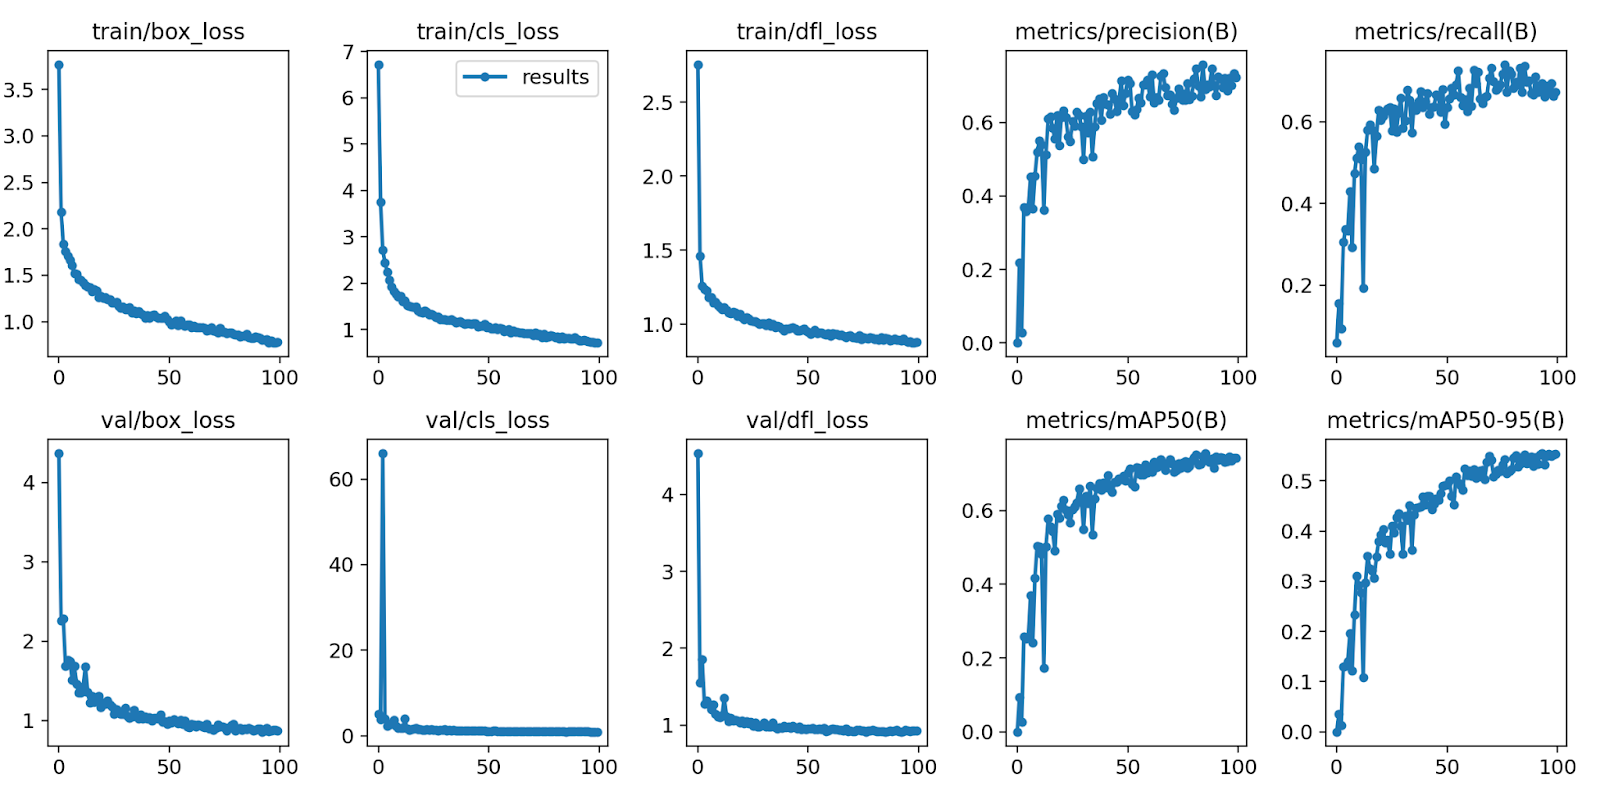
\includegraphics[width=14cm]{images/loss-function-distillation.png}
% \begin{center}
%     Fig(13) Result without Distillation
% \end{center}

% 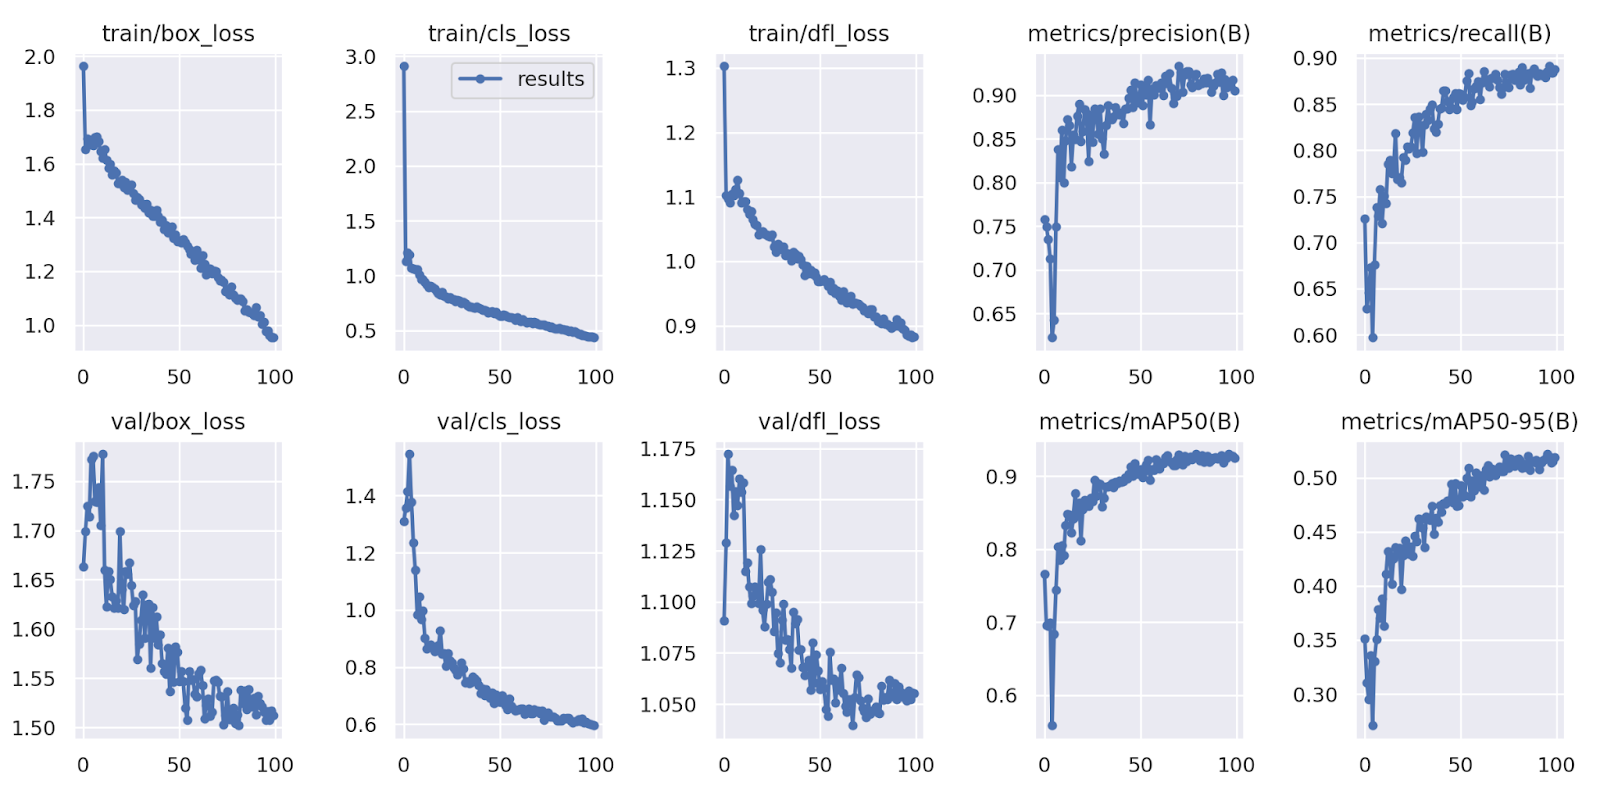
\includegraphics[width=14cm]{images/loss-function-without-distillation.png}
% \begin{center}
%     Fig(14) Result without Distillation
% \end{center}


% \documentclass{article}
% \usepackage{graphicx}
% \usepackage{subcaption}

% \begin{document}

% \begin{figure}[ht]
%   \subcaptionbox*{First subfigure}[.45]{%
%     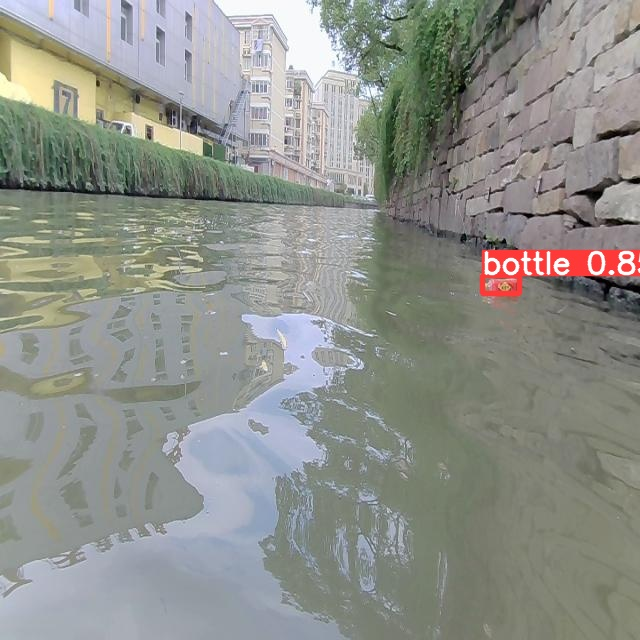
\includegraphics[width=5cm]{images/test-img-1.png}%
%   }%
%   \hfill
%   \subcaptionbox*{Second subfigure}[.45]{%
%     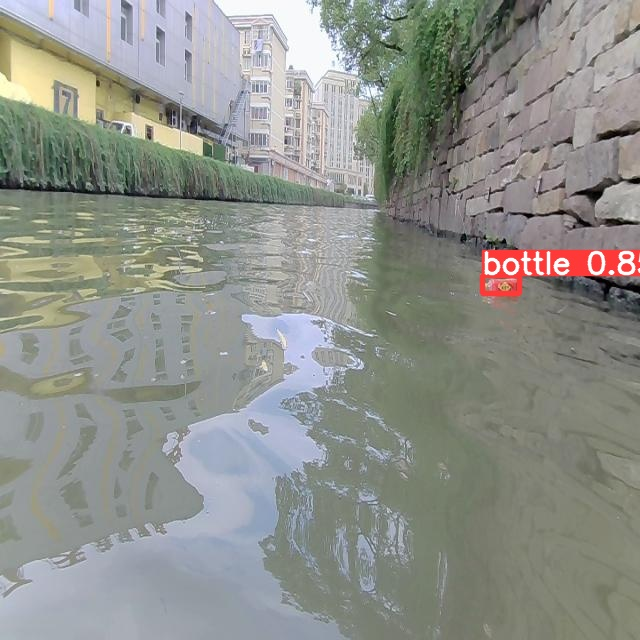
\includegraphics[width=5cm]{images/test-img-1.png}%
%   }
%   \caption{Two images}
% \end{figure}


% \end{document}

\end{enumerate}
\begin{table}[H]
    \centering
 
\begin{tabular}{lccr}
\hline \multicolumn{1}{c}{Model} & Dataset & mAP50-95 & FPS\\
\hline DSSD & $FloW $ & 27.5 \% & 28.6\\
RetinaNet & $FloW $  & 24.9 \% & 7.6\\
YOLO-v3 & $FloW $ & 12.8 \% & 23.2\\
Faster R-CNN & $FloW $ & 18.4 \%  & 9.3\\
FPN & $FloW $ & 33.4 \% & 7.4\\
Cascade R-CNN & $FloW $ & 43.4 \% & 3.9\\
YOLOv5 & $FloW $ & 50.2 \% & 31\\
\textbf{YOLOv8} & \textbf{$FloW$}  & 55.2\% & \textbf{57.14}\\
\textbf{DistilledFloatNet} & \textbf{$FloW$} & 55.4\% & \textbf{78.74}\\
\hline
\end{tabular}
\caption{Comparison with other Models}
   \label{table:training-3}
\end{table}

\vspace{\baselineskip}
\vspace{\baselineskip}
\begin{figure}[H]
\centering
\subcaptionbox{}
{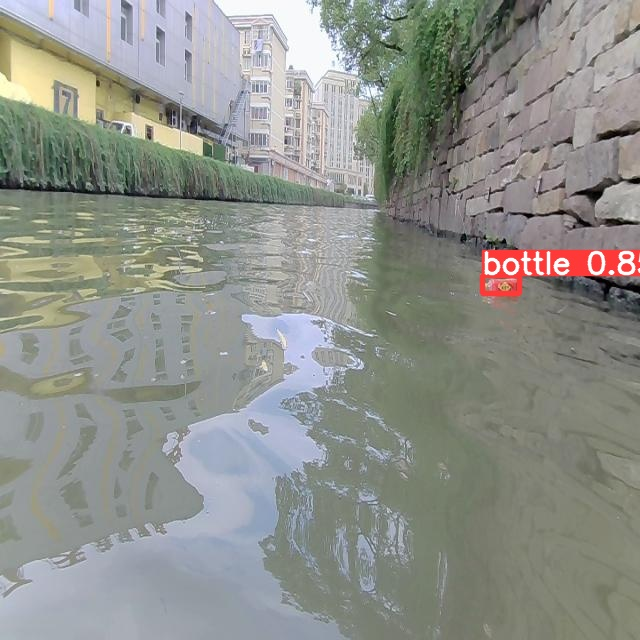
\includegraphics[width=0.45\textwidth]{images/test-img-1.png}}%
\hfill % <-- Seperation
\subcaptionbox{}
{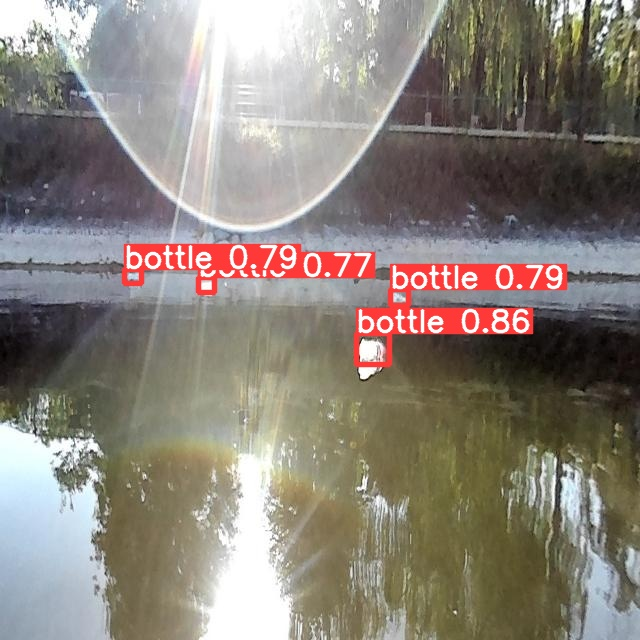
\includegraphics[width=0.45\textwidth]{images/test-image-2.png}}%
\caption{Test Images}
\label{fig:test}
\end{figure}

% \begin{figure}[H]
% \centering
% \subcaptionbox{Subcaption A}{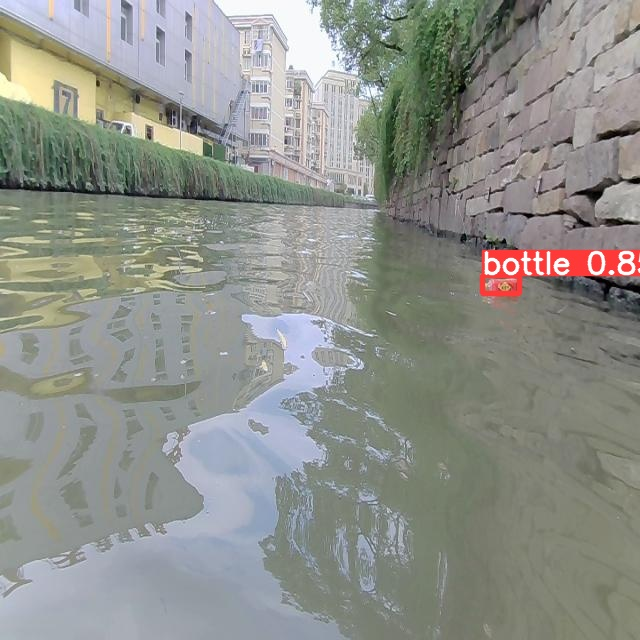
\includegraphics[width=0.30\textwidth]{images/test-img-1.png}}%
% \hfill
% \subcaptionbox{Subcaption B}{\includegraphics[width=0.30\textwidth]{images/test-img-2.png}}%
% \caption{Caption}
% \label{fig:nmbdmbkd}
% \end{figure}

%     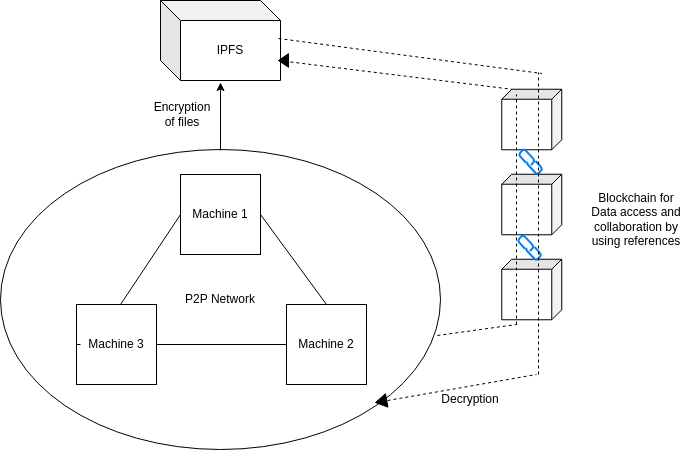
\includegraphics[width=14cm]{images/arch.png}
% \begin{center}
%     Proposed System Design
% \end{center}

% \newpage
% \section{Gantt Chart of Progress}
% \noindent\\\\
%     % \centering
%     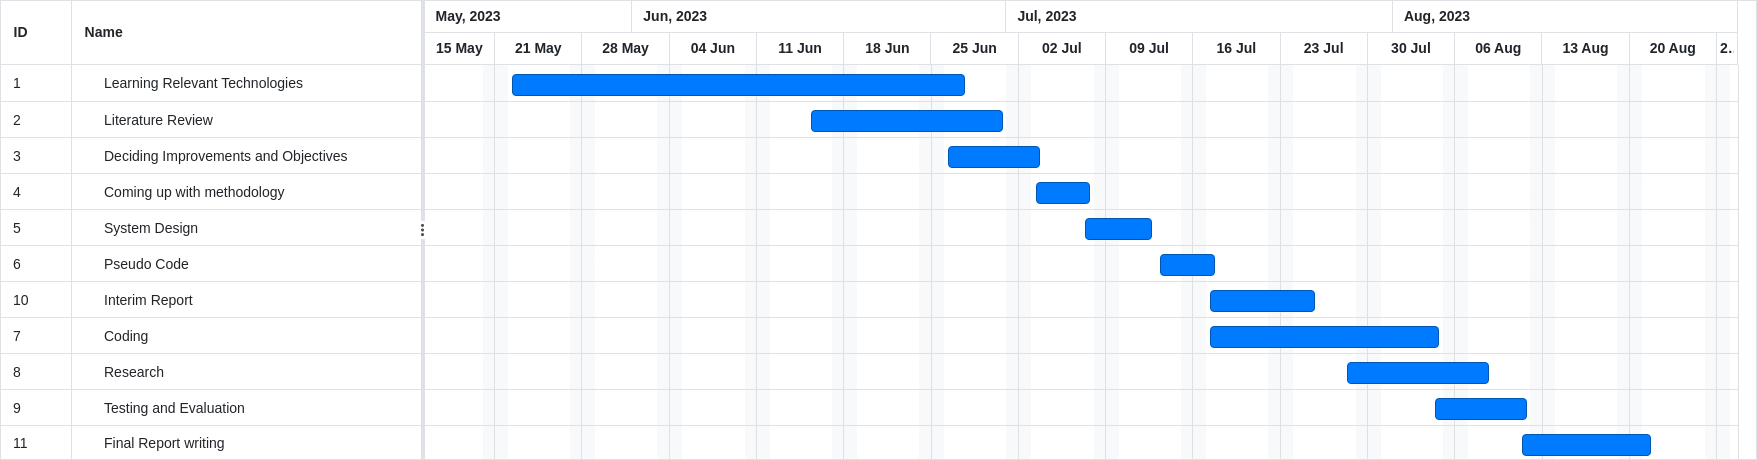
\includegraphics[width=16cm]{images/gantt.png}
% \subsection{Neural Network Architecture for Image Description Generation}
% \noindent The current study involves designing the architecture of the image description generation module using the encoder-decoder based method. Encoder will output the feature vector after taking image as the input. The feature vector will be given to the attention module and then a simple and efficient decoder will be selected to output the sequence of words as the image description. An overview of the proposed architecture is given in the figure \ref{fig:Chapter-4d}.

% \begin{figure}[h]
% \centering
% 	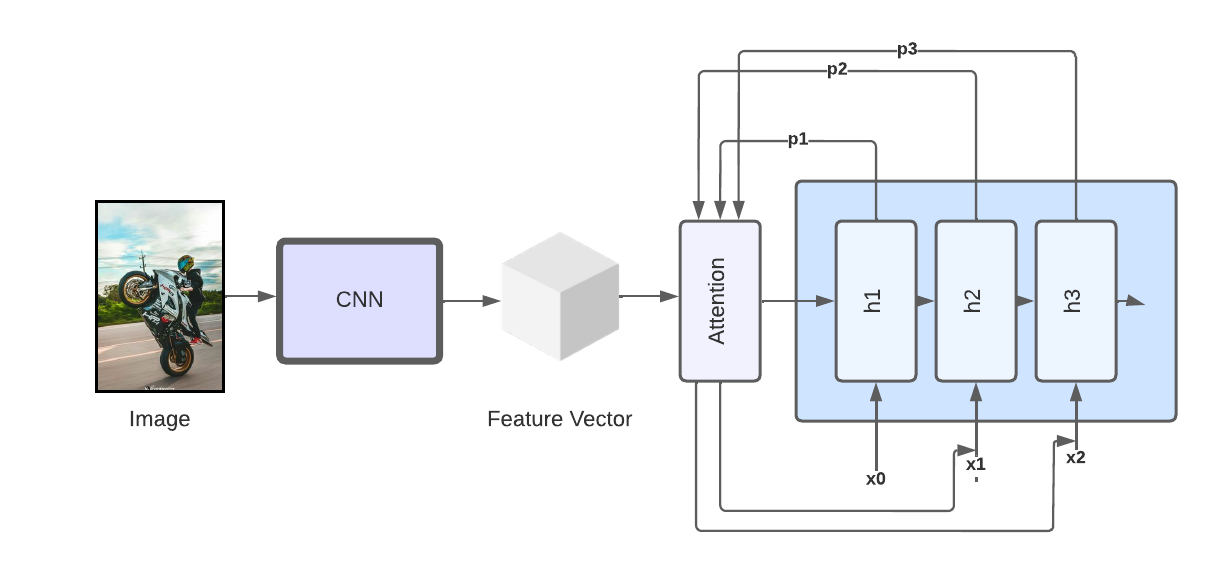
\includegraphics[scale=0.8]  {chapters/4/intfig/attention.png}
% 	  \caption{An overview of the proposed architecture of the image description generation module.}
% 	\label{fig:Chapter-4d}
% \end{figure}

% \noindent The encoder (CNN) in Figure \ref{fig:Chapter-4d} will return a feature vector of image which will be fed as input to the attention module. The attention module will compute attention weights for each iteration using the context and the feature vector. The attention weights will be multiplied with the feature vector and then will fed to sequence model (LSTM/GRU).

% \subsection{Automating Encoder Selection}
% \noindent There are various encoders that can be used to fetch the image vector representation. To deal with the uncertainty of the selection of encoder which gives the best result for image description generation. We will deploy all the models with various encoders and automate the selection of the encoder based on the matching labels obtained from object/label detection algorithm.
% \begin{figure}[h]
% \centering
% 	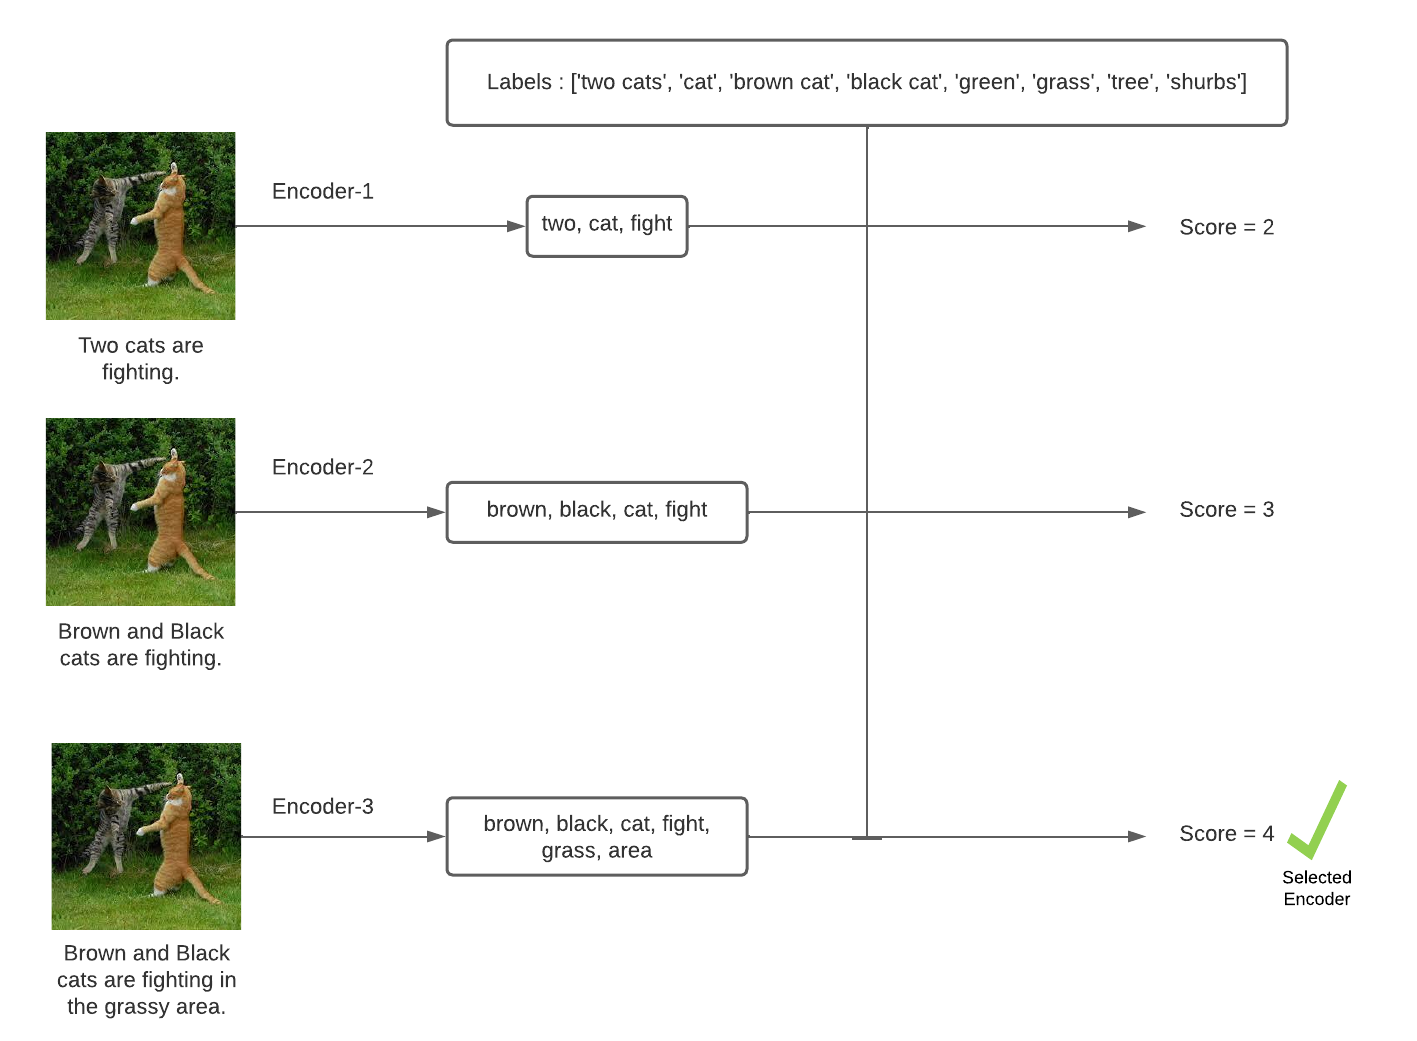
\includegraphics[scale=0.7]{chapters/4/intfig/automate.png}
% 	  \caption{Automating the selection of different encoders based on the labels obtained from the object detection algorithm.}
% 	\label{fig:Chapter-4d-automate}
% \end{figure}

% \noindent Figure \ref{fig:Chapter-4d-automate} describes, the method for automating the object detection. The labels will be generated by the object detection and caption will be generated by the various encoder-decoder model. Root word will be extracted from the captions and the score will be calculated based on number of root word matching with the labels. The model with the best score will be selected for sending the image description.

% \subsection{Design for Native Mobile Application}
% \noindent After, we have our efficient and simple model for generating image description. We will deploy our model on the cloud platform and will build an mobile application that will help the blind individual to click a photo and get the audio of the image description generated. 

% \begin{figure}[h]
% \centering
% 	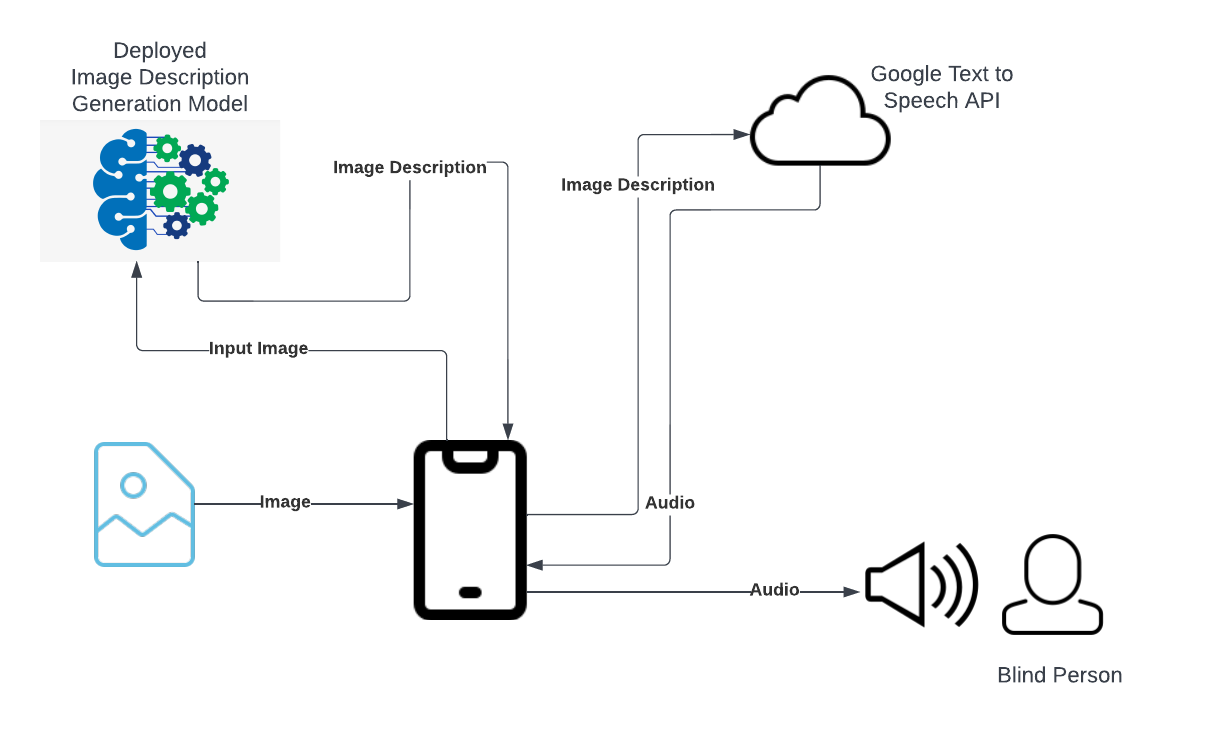
\includegraphics[scale=1.0]  {chapters/4/intfig/system_design.png}
% 	  \caption{An overview of the proposed architecture of the image description generation module.}
% 	\label{fig:Chapter-4d-system_design}
% \end{figure}

% \noindent The flow of the logic of the system described in the Figure \ref{fig:Chapter-4d-system_design} is as follows:
% \begin{enumerate}
%     \item The input will be taken from the native mobile application.
%     \item The user will request for the description of the image from the deployed ML model on the cloud.
%     \item The model will return the description sentence to the client side of the application.
%     \item Google's Text to Speech API will be used to convert the image's description to the audio.
%     \item The audio will be played for the blind person to tell them about the description of the image.
% \end{enumerate}
% % \noindent The first step required to establish a research in this area is to give input images, that are to be passed through a preprocessing phase. Preprocessing of images includes scaling, shifting, rotating etc. as per the  requirement on those particular images. Preprocessing also includes conversion of images such as from RGB to grayscale. Furthermore, at the processing stage itself filtering of noise is also established. After preprocessing comes the process of extraction of features from the image and the background. Extraction of features can be obtained from various means of skin segmentation, using various techniques. Followed by extraction of features comes modeling of features that is enhancing the discriminative powers of essential parameters for better processing and results. Then comes the phase of skin classification where the skin pixels are segregated into two parts that is skin pixels and non-skin pixels.
% % \begin{figure}[h]
% % \centering
% % 	\includegraphics*[height = 11cm, width = 13cm]{chapters/1/intfig/Block_diagram2.eps}
% % 	 \caption{Block diagram of our proposed methodology.}
% % 	\label{fig:Chapter-4a}
% % \end{figure}
% % \section{Work Done} 
% % We test the basics color models.That gives us the result.We obtain that the all these models insuficent to get the skin at same parameters. result will be shown in fig(i).
% % begin{figure}[h]
% % \centering
% % \includegraphics*[height = 11cm, width = 13cm]{chapters/1/intfig/Block_diagram2.eps}
% \newpage
% \section{Proposed methodology}
% \noindent The objective of the present study is to generate image description with good performance. The task of generating the image caption can be divided into two parts:
% \begin{enumerate}
%     \item Feature Extraction
%     \item Description Generation
% \end{enumerate}

% \subsection{Feature Extraction}
% \noindent Most of the studies conducted on image captioning have proved that encoder-decoder based architecture gives a rich description of the image with high performance. The three dimensional image is given as input to the encoder part of the architecture and image's feature representation is extracted as output of the encoder. Convolutional Neural Network (CNN) serves the purpose of the encoder. Generally, CNN performs manipulations on the image using the Convolution layer and Pooling Layer. It effectively reduces the dimensionality of the image without losing the necessary information or features captured in the image. Many pre-trained Convolutional Neural Network based architecture (ResNet, VGG, Inception) are present, which can reduce the time of training the image description generation model. \\
% The first task is to choose an efficient CNN model, considering the complexity and the performance of various CNN models. The parameters, accuracy and depth of the network of various CNN models is given in the Table \ref{table:1}. \\

% \begin{table}[h!]
%     \centering
%     \caption{CNN Models Accuracy, Parameters, Layers}
%     \begin{tabular}{ |c|c|c|c|c| } 
%      \hline
%      \textbf{S.No.} & \textbf{CNN Model} & \textbf{No. of Parameters} & \textbf{No. of Layers} & \textbf{Accuracy on ImageNet}\\ 
%      \hline
%      1 & VGG16 & 138,35,544 & 16 & 74.5\% \\ 
%      2 & Inception V3 & 23,851,784 & 42 & 78.8\% \\
%      3 & ResNet50 & 23,587,712 & 50 & 77.6\% \\
%      \hline
%     \end{tabular}
%     \label{table:1}
% \end{table}

% \newpage
% \subsubsection{VGG16}
% \noindent Visual Geometry Group (VGG) is a Convolutional Neural Network (CNN) architecture proposed by Karen {\em{et al.}} \cite{vgg}. VGG16 has 16 number of layers where weights are learned while training the model. VGG19 is also a Convolutional Neural Network model available which has 19 layers with weights. \\
% The VGG16 model takes a standard input image with size 244x244x3. It uses kernel filter of 3x3 size with stride 1. They use maxpool of size 2x2 with stride 2. The size of the kernel filter, maxpool filter and padding is constant throughout the model. The detailed architecture of VGG16 is given in the figure \ref{fig:vgg16_architecture}. 

% \usetikzlibrary{positioning,fit,calc}
% \tikzset{block/.style={draw, thick, text width=6cm, minimum height=0.5cm, align=center},   
% line/.style={-latex}
% }  

% \begin{figure}
%     \centering
%     \begin{tikzpicture}   
%       \node[block] (o) {\small Output};  
%       \node[block] (n) at ([yshift=-0.9cm]$(o)$) {\footnotesize Softmax};  
%       \node[block] (m) at ([yshift=-0.9cm]$(n)$) {\footnotesize Fully Connected};  
%       \node[block] (l) at ([yshift=-0.9cm]$(m)$) {\footnotesize Fully Connected};  
%       \node[block] (k) at ([yshift=-0.9cm]$(l)$) {\footnotesize Max Pooling};  
%       \node[block] (j) at ([yshift=-0.9cm]$(k)$) {\footnotesize 3 x Convolution 512};  
%       \node[block] (i) at ([yshift=-0.9cm]$(j)$) {\footnotesize Max Pooling};  
%       \node[block] (h) at ([yshift=-0.9cm]$(i)$) {\footnotesize 3 x Convolution 512};  
%       \node[block] (g) at ([yshift=-0.9cm]$(h)$) {\footnotesize Max Pooling};  
%       \node[block] (f) at ([yshift=-0.9cm]$(g)$) {\footnotesize 3 x Convolution 256};  
%       \node[block] (e) at ([yshift=-0.9cm]$(f)$) {\footnotesize Max Pooling};  
%       \node[block] (d) at ([yshift=-0.9cm]$(e)$) {\footnotesize 2 x Convolution 128};  
%       \node[block] (c) at ([yshift=-0.9cm]$(d)$) {\footnotesize Max Pooling};  
%       \node[block] (b) at ([yshift=-0.9cm]$(c)$) {\footnotesize 2 x Convolution 64};  
%       \node[block] (a) at ([yshift=-0.9cm]$(b)$) {\footnotesize Input Image};   

%       \node[right=of a] {\footnotesize 244 x 244 x 3};
%       \node[right=of b] {\footnotesize 244 x 244 x 64};
%       \node[right=of c] {\footnotesize 112 x 112 x 64};
%       \node[right=of d] {\footnotesize 112 x 112 x 128};
%       \node[right=of e] {\footnotesize 56 x 56 x 128};
%       \node[right=of f] {\footnotesize 56 x 56 x 256};
%       \node[right=of g] {\footnotesize 28 x 28 x 256};
%       \node[right=of h] {\footnotesize 28 x 28 x 512};
%       \node[right=of i] {\footnotesize 14 x 14 x 512};
%       \node[right=of j] {\footnotesize 14 x 14 x 512};
%       \node[right=of k] {\footnotesize 7 x 7 x 512};
%       \node[right=of l] {\footnotesize 4096};
%       \node[right=of m] {\footnotesize 4096};
%       \node[right=of n] {\footnotesize 1000};

      
%       \draw[line] (a)-- (b);
%       \draw[line] (b)-- (c);
%       \draw[line] (c)-- (d);
%       \draw[line] (d)-- (e);
%       \draw[line] (e)-- (f);
%       \draw[line] (f)-- (g);
%       \draw[line] (g)-- (h);
%       \draw[line] (h)-- (i);
%       \draw[line] (i)-- (j);
%       \draw[line] (j)-- (k);
%       \draw[line] (k)-- (l);
%       \draw[line] (l)-- (m);
%       \draw[line] (m)-- (n);
%       \draw[line] (n)-- (o);
%     \end{tikzpicture}  
%     \caption{The architecture of the pre-trained CNN model, VGG16 \cite{vgg}}
%     \label{fig:vgg16_architecture}
% \end{figure}

% \subsubsection{Inception}
% \noindent Inception V3 is also a CNN pre-trained model published in 2015 \cite{inception}. It performed better than its subsequent parts like V1 and V2. There were many major advancements that led to increase in the performance of Inception V3. It factorized the convolutions into many smaller convolutions, a convolution was spillted to many asymmetric convolution to reduce the computation. In total, the Inception V3 consisted of 42 layers. A constrained view of the Inception model is given in the figure \ref{fig:inceptionv3_architecture}.
% \begin{figure}[h!]
%     \centering
%     \begin{tikzpicture}   
%       \node[block] (o) {\small Output};  
%       \node[block] (n) at ([yshift=-0.9cm]$(o)$) {\footnotesize Softmax};  
%       \node[block] (m) at ([yshift=-0.9cm]$(n)$) {\footnotesize Fully Connected};  
%       \node[block] (l) at ([yshift=-0.9cm]$(m)$) {\footnotesize Global Avg. Pooling};  
%       \node[block] (k) at ([yshift=-0.9cm]$(l)$) {\footnotesize 2 x Inception C};  
%       \node[block] (j) at ([yshift=-0.9cm]$(k)$) {\footnotesize Reduction B};  
%       \node[block] (i) at ([yshift=-0.9cm]$(j)$) {\footnotesize 4 x Inception B};  
%       \node[block] (h) at ([yshift=-0.9cm]$(i)$) {\footnotesize Reduction A};  
%       \node[block] (g) at ([yshift=-0.9cm]$(h)$) {\footnotesize 3 x Inception A};  
%       \node[block] (f) at ([yshift=-0.9cm]$(g)$) {\footnotesize Max Pooling 3*3/2};  
%       \node[block] (e) at ([yshift=-0.9cm]$(f)$) {\footnotesize Convolution 3*3 (192/1)};  
%       \node[block] (d) at ([yshift=-0.9cm]$(e)$) {\footnotesize Convolution 1*1 (80/1)};  
%       \node[block] (c) at ([yshift=-0.9cm]$(d)$) {\footnotesize Max Pooling 3*3/2};  
%       \node[block] (b) at ([yshift=-0.9cm]$(c)$) {\footnotesize 3 x Convolution 3*3};  
%       \node[block] (a) at ([yshift=-0.9cm]$(b)$) {\footnotesize Input Image};   

%       \node[right=of a] {\footnotesize 299 x 299 x 3};
%       \node[right=of b] {\footnotesize 147 x 147 x 64};
%       \node[right=of c] {\footnotesize 73 x 73 x 64};
%       \node[right=of d] {\footnotesize 73*73*80};
%       \node[right=of m] {\footnotesize 2048};
%       \node[right=of n] {\footnotesize 1000};

      
%       \draw[line] (a)-- (b);
%       \draw[line] (b)-- (c);
%       \draw[line] (c)-- (d);
%       \draw[line] (d)-- (e);
%       \draw[line] (e)-- (f);
%       \draw[line] (f)-- (g);
%       \draw[line] (g)-- (h);
%       \draw[line] (h)-- (i);
%       \draw[line] (i)-- (j);
%       \draw[line] (j)-- (k);
%       \draw[line] (k)-- (l);
%       \draw[line] (l)-- (m);
%       \draw[line] (m)-- (n);
%       \draw[line] (n)-- (o);
%     \end{tikzpicture}  
%     \caption{The architecture of the pre-trained CNN model, Inception V3 \cite{inception}}
%     \label{fig:inceptionv3_architecture}
% \end{figure}

% \subsubsection{ResNet50}
% \noindent The ResNet architecture was proposed to solve the problem of the vanishing gradient commonly seen in the CNN models. The problem was resolved using the skip connections between the different layers \cite{resenet}. ResNet50 architecture was 50 layers deep and had fewer parameters than the VGG16 and Inception V3 architecture. Though, the model will be difficult to train because of the increase in the depth but will certainly have better performance. The architecture of ResNet50 is given in the figure \ref{fig:resnet}.
% \begin{figure}[h!]
% \centering
% 	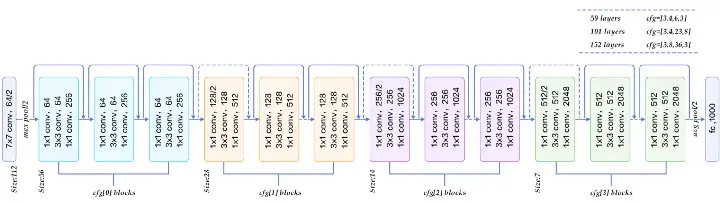
\includegraphics[scale=0.7]  {chapters/4/intfig/resnet.png}
% 	  \caption{The architecture of the pre-trained CNN model, ResNet50 \cite{resenet}}
% 	\label{fig:resnet}
% \end{figure}
% \subsubsection{Feature Vector Representation of Image}
% \noindent Consider, image $I$ is fed into any selected convolutional neural network model. The output of the encoder will be the visual representation of the features of the image. Let's say $F$ is the feature vector received as output after fully connected layer of CNN and $V$ is the spatial vector received as output from the last convolution layer of CNN.
% \begin{equation}
%     F = C_{fc}(I)
% \end{equation}
% \begin{equation}
%     V = C_{conv}(I)
% \end{equation}

% \noindent Here, $C_{fc}$ is the output of the fully connected later of CNN and $C_{conv}$ is the output of the last convolution later of CNN.
% \begin{equation}
%     V=\{v_{1}, v_{2}, ...., v_{k^2}\}
% \end{equation}
% The output of the last convolution layer $V$ is the visual $k$ x $k$ grid which can map to the previous convolution layer outputs and can perfectly define the relative feature positions. \\
% The fully connected layer output $F$ will be given as input to the decoder or language model in model where no attention mechanism is adopted, while the $F$ will be the input to the attention module in the attention mechanism model of image description generation.

% \subsection{Description Generation}
% \noindent The task of image description generation deals with the generation of sequence of words. The idea of generation of sequence of words make us use the Recurrent Neural Network (RNN). \\
% Consider $I$ is the input image and $\theta$ is the model parameter to be trained. The aim of the model is to generate sentence $S$ by maximising the likelihood of the expression.
% \begin{equation}
%     \theta^{*} = \arg \max_{\theta} \sum (I,S) \log p(S|I;\theta)
% \end{equation}
% \begin{equation}
%     h_{t+1} = f(h_{t},x_{t})
% \end{equation}
% The generation of the next hidden state $(h_{t+1})$ is a non-linear function $(f)$ of the previous hidden state and the context word $(h_{t})$. The naive RNN network fails to deal with the long sequence of words because of the exploding gradients words get vanished with time. Many researches conducted on image caption generation adopted LSTM as the language generation model as it solves the problem discussed aforementioned. \\
% In our study we will be experimenting with both LSTM and GRU model. GRU is simpler RNN model with not only solves the above mentioned problem but also requires lesser parameter to train. It is an effort to reduce the complexity of the decoder section of the architecture. 
% \subsubsection{LSTM - Long Short-Term Memory}
% \begin{figure}[h]
% \centering
% 	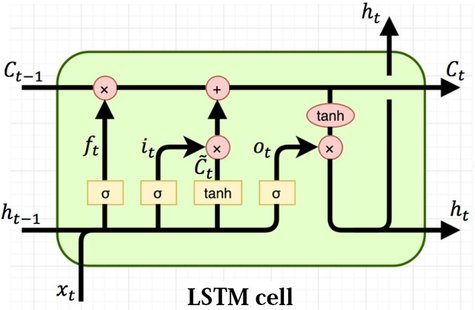
\includegraphics  {chapters/4/intfig/lstm.png}
% 	  \caption{The basic architecture of the repeating module of LSTM \cite{lstm}}
% 	\label{fig:Chapter-4a}
% \end{figure}
% \noindent LSTM is a variation of the recurrent neural network. It consist of three gates: input gate, output gate and the forget gate. The value of previous hidden state, $h_{t-1}$ and the current element of the sentence $x_{t}$ is passed through the sigmoid function.
% \begin{equation}
%     f_{t} = \sigma(W_{f}.[h_{t-1},x_{t}]+b_{f})
% \end{equation}
% Now, we need to decide through the input layer, $i_{t}$ which values needs to be updated and set of all the possible candidates that could be the next potential $C_{t}$.
% \begin{equation}
%     i_{t} = \sigma(W_{i}.[h_{t-1},x_{t}]+b_{i})
% \end{equation}
% \begin{equation}
%     \Tilde{C_{t}} = \tanh(W_{C}.[h_{t-1},x_{t}]+b_{c})
% \end{equation}
% $C_{t-1}$ will be updated to $C_{t}$ using the formula given below.
% $$C_{t} = f_{t}*C_{t-1} + i_{t}*\Tilde{C_{t}}$$
% The output of the hidden state of this iteration will be decided using the sigmoid and the hyperbolic function.
% \begin{equation}
%     o_{t} = \sigma(W_{o} [h_{t-1},x_{t}] + b_{o})
% \end{equation}
% \begin{equation}
%     h_{t} = o_{t}*\tanh(C_{t})
% \end{equation}

% \noindent The $C{t}$ and $h_{t}$ will be fed as input to the LSTM at $t+1$ iteration. At every iteration, the $h_{t}$ given to the softmax function to get the distribution of probability of every word from the dataset. 
% \subsubsection{GRU - Gated Recurrent Unit}
% \begin{figure}[h]
% \centering
% 	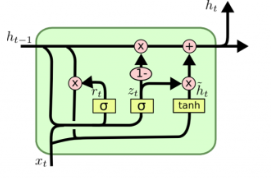
\includegraphics  {chapters/4/intfig/gru.png}
% 	  \caption{The basic architecture of the repeating module of GRU \cite{gru}}
% 	\label{fig:Chapter-4a}
% \end{figure}
% \noindent GRU is also a version of recurrent neural network solving the problem of long-term dependency very efficient. The model is not very complex and requires lesser parameters to be trained than the LSTM model. The GRU architecture only gives the hidden state $h_{t}$ and no $C_{t}$ as the output. This architecture is faster to train. This network contains: update gate $(z_{t})$ and reset gate $(r_{t})$. These gates decide the value of the hidden state $(h_{t})$ that will given as input to the GRU for next iteration.
% \begin{equation}
%     z_{t} = \sigma(W_{z}x_{t} + U_{z}h_{t-1}+b_{z})
% \end{equation}
% \begin{equation}
%     r_{t} = \sigma(W_{r}x_{t} + U_{r}h_{t-1}+b_{r})
% \end{equation}
% \begin{equation}
%     h_{t} = (1-z_{t}) \cdot h_{t-1} + z_{t} \cdot \tanh(W_{h}x_{t} + U_{h}(r_{t}\cdot h_{t-1}) + b_{h})
% \end{equation}

% \noindent At every iteration, the $h_{t}$ given to the softmax function to get the distribution of probability of every word from the dataset. 
% \subsection{Visual Attention}
% \begin{figure}[h]
% \centering
% 	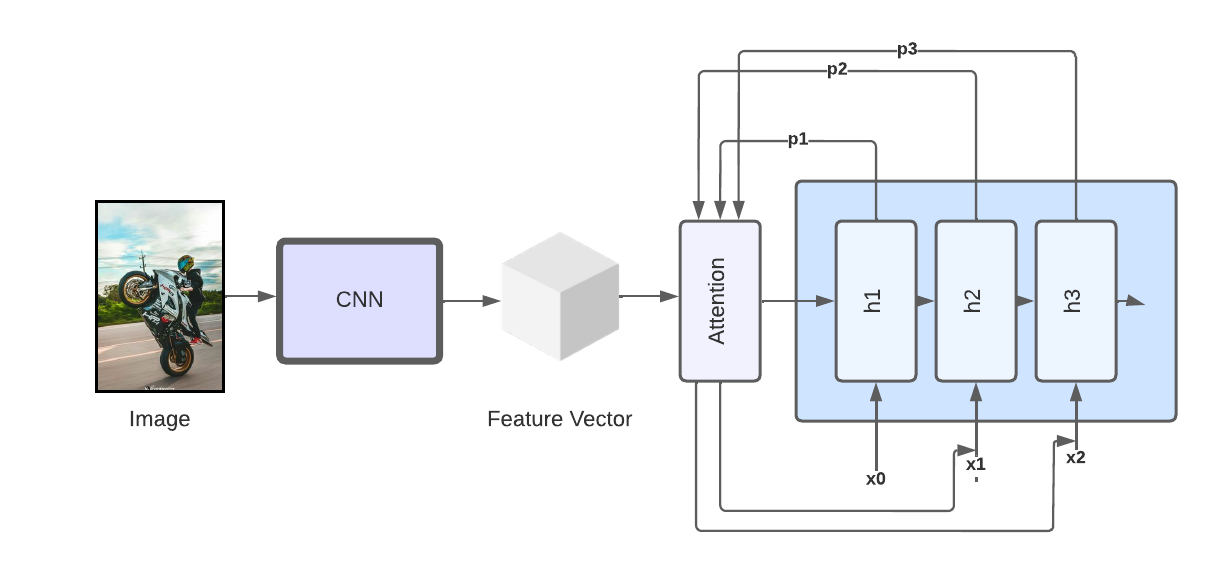
\includegraphics[scale=0.8]  {chapters/4/intfig/attention.png}
% 	  \caption{Encoder-Decoder based architecture for image description generation using attention module}
% 	\label{fig:Chapter-4a}
% \end{figure}
% \noindent The idea of the attention mechanism comes from the attention used for the image classification, as all of the pixels are of no use to classify the image. In attention-based image description generation, the output of the convolutional fully connected layer fed into the attention module. With attention gate, the decoder concentrate on only those pixel of the image that are relevant. In each iteration, the feature vector representation of the image and previous context of the LSTM or GRU is given to the attention module. The attention module then calculates the weight of the attention vector. The attention mechanism is differentiable. The training of the attention mechanism can be done using the backpropagation.
% \begin{equation}
%     a_{t} = \sum_{1}^{n} S_{j}Y_{j}
% \end{equation}
% Here, $a_{t}$ is the attention vector obtained after training. $S$ is the function that gives the output after performing the softmax operation. $Y$ is the feature representation of the image.


% \section{Evaluation metrics}
% \noindent The description of the images generated needs to be rich in the information displayed, readable and grammatically correct. This is a supervised learning module where we have the predicted description along with the reference description. The evaluation metrics measures how much the predicted description matches with the true description. In our study, we will be checking the performance of our model on evaluation metric like BLEU, GLEU, METEOR. \\
% BLEU score is evaluated by first calculating the n-gram of the predicted description and the true description \cite{bleu}. Then it counts the matching in the respective n-grams. This score was majorly defined to evaluate the performance of the translation of the languages model. The structure of the description is not taken into consideration in the BLEU score. A model should achieve atleast a BLEU score of more than 0.5 for valid consideration. \\
% METEOR score worked on the disadvantage of the BLEU score. This evaluation metric uses the WordNet for matching the resemblance between the predicted description and true description. It also calculates the resemblance between the synonyms, suffix, prefix and the roots of the sentences, making it closer to the human discrimination \cite{meteor}.
% \begin{equation}
%    METEOR = 10* Precision * \frac{Recall}{Recall + 9 * Precision} 
% \end{equation}
% METEOR uses the Precision and Recall to calculate the score. Recall is given more weightage than the Precision making it more closer to the human description. \\
% GLEU is another evaluation metric to check the performance of the image description module with respect to the grammatical errors and the fluency of the generated sentences. The n-gram of the generated description is overlapped with the different sentences. GLEU score is identical to the BLEU score with respect to the computation.


% \section{Dataset}
% \noindent \textbf{Flickr8k} dataset will be used to evaluate the performance of the image description generation and also for training the model. The dataset consist of 8000 images which can be splitted in the ratio of 6:1:1 for training, validation and testing purpose respectively. In the dataset, for each and every image there are five descriptions. There is also Flickr30k dataset which consist of 30,000 images in total. The performance of the model will increase with the number of the images used for training the model. So, Flickr30k dataset will be used to improve the performance of the model \cite{flickr30k}.\\
% \noindent \textbf{MSCOCO} dataset is also similar with respect to the structure, it also contains five descriptions for each image. Total number of images in the dataset is around 164K. The training set can have 84K images, validation set and testing set can contain 40K images each \cite{mscoco}. Due, to hardware constraint we will restrict our training with Flickr dataset. 

% \section{Text-To-Speech (TTS) Conversion}
% \noindent In our study, the description obtained from the neural network model will be converted to the waveforms, audio for assisting the blind person about the image. We will be using Google's Text-To-Speech API for performing the mentioned task. \\
% The API works on the Tacotron 2 \cite{tacotron2}, proposed by the engineers of Google. It is a neural network architecture for generating the audio version of the text (speech synthesis). The neural network architecture works on Seq2Seq model, where inputs are the sequence of word embeddings and output is mel-scale spectrograms, which is sequence of waveforms for audio. The architecture comprises of two major components, (i) RNN Seq2Seq Model with attention module which takes input as the sequence of words and produces mel spectrogram sequence, and (ii) WaveNet \cite{wavenet} which takes predicted mel spectrogram frames as input and convert it to waveforms for raw audio which is much more closer to the human speech. This model achieved mean opinion score(MOS) of 4.53 much closer to professional human speech.